\section{Several Random Variables (and related things)} \label{s9} 

\ssn{Learning Outcomes}
After studying this week you will be able to:
\begin{itemize}
\item calculate probabilities and marginal densities from joint densities;  
\item use joint densities to solve some problems involving more than one random variable. 
\end{itemize}
\end{n}

\subsection{Preparation for the week}



\ssn{Motivating problems}
\begin{itemize}
\item How can we work with several random variables at once? 
\item A unit length, thin rod breaks in two places, each break independently uniformly distributed on $(0,1)$.  What is the probability that the breaks are more than distance $0.5$ apart? 
\item I choose five numbers in $[0,1]$ uniformly randomly. What is the expected position of the second smallest number? 
\end{itemize}
\end{n}



\ssn{Magic coins}
\begin{table}[h] 
\centering  \[  \arraycolsep=6pt\def\arraystretch{2.0} 
\begin{array}{|c|cc|}
 \hline 
   & X=H & X=T \\ 
  \hline
Y=H &  \frac4{12} & 
      \frac1{12}    \\
Y=T &  \frac2{12} & \frac5{12}  \\
\hline
\end{array} \quad 
\begin{array}{|c|cc|}
 \hline 
   & \PP(X=H)=\frac12 & \PP(X=T)=\frac12 \\
  \hline
\PP(Y=H)=\frac5{12} &  \frac4{12} & 
      \frac1{12}    \\ 
\PP(Y=T)=\frac7{12} &  \frac2{12} & \frac5{12}  \\
\hline
\end{array}
\] 
\caption{Pair of magic coins. (The numbers mean that e.g.\ the probability of both being T is $5/12$.) On the left the probability of all the outcomes is given. In the version on the right the ``marginal probabilities'' for $X$ and $Y$ have been added. \label{mc1}}
\end{table}

My two magic coins $X$ and $Y$ come down with probabilities as in the left-hand side of Table~\ref{mc1}; the four probabilities add up to $1$, as they should.   From that data, we can compute the probabilities that each of the coins separately comes down H or T by adding up each row and column; that information has been added to the table on the right.   But $\PP( \text{$X=H$ and $Y=H$}) \not= \PP(X=H)\, \PP(Y=H)$: the first coin and the second are not independent. 
\end{n}

\ssn{The discrete case}  \label{jdisc} 
Consider two discrete random variables $X,Y$ which for simplicity we assume take values in the non-negative integers $0,1,2,\dots$.   (Each may take infinitely many values (e.g.\ geometric or Poisson) or just a finite number of them (e.g.\ binomial).) 

\tcb 
The \emph{joint probability mass function} of $X,Y$ is 
 \[
      p_{X,Y}(x,y) = \PP(\text{$X=x$ and $Y=y$}). 
 \]
 \etcb 
 
 \noindent
To be valid, we need only to know that 
  \[
    0 \leq p_{X,Y}(x,y) \leq 1 \;\text{ for all $x,y$ } \quad \text{ and } \quad \sum_x \sum_y p_{X,Y}(x,y) = 1. 
   \] 
 
\tcb 
The \emph{marginal mass functions} of $X,Y$ are defined by 
 \[
     p_X(x) = \sum_y p_{X,Y}(x,y)  \quad \text{ and } \quad  p_Y(y) = \sum_x p_{X,Y}(x,y). 
 \]
 \etcb 
 
 \noindent
 They tell us the distribution of each variable, ignoring the other one. 
Clearly, one can extend the definitions to three or more random variables. 
\end{n}

\sse{} 
Prove that the joint mass function $p_{X,Y}$ satisfying the two conditions in \S\ref{jdisc} implies that the marginal distributions satisfy the conditions to be probability mass functions.  
\end{e}

\ssn{The continuous case}
For one continuous random variable $X$ we have a density function $f_X(x)$. It is such that in the limit as  $\Delta x \map 0$ we have 
 \[
    \PP( x \leq X \leq x + \Delta x ) = f_X(x) \Delta x. 
 \]

Two continuous random variables $X,Y$ can be thought of as defining a random point $(X,Y)$ in the plane. A continuous random variable is described by a probability density function $f_{X,Y}$ taking non-negative values so that in the limit as $\Delta x \map 0$ and $\Delta y \map 0$ we have 
 \[
    \PP( \text{$x \leq X \leq x + \Delta x$ and 
    $y \leq Y \leq y + \Delta y$}) = f_X(x,y) \Delta x \Delta y. 
 \]

With our usual convention that the density function is taken to be zero outside of the region where $(X,Y)$ takes values, we require that 
 \[
      \int \int_{\mathbb R^2} f_{X,Y}(x,y) \, \dd x \dd y = 1
 \]
One case is where $f_{X,Y}(x,y) = k$ for all points in some region $D$ in the plane and zero outside. 
This corresponds to choosing a point $(X,Y)$ uniformly randomly in the region $D$.  The constant in that case is $k= 1/\mathop{Area}(D)$ and the probability that $(X,Y)$ lies in a particular (sensibly-shaped) region  $A \subseteq D$ is 

\tcb
 \[
  \PP( (X,Y) \in A) = \frac{\mathop{Area}(A)}{\mathop{Area}(D)}.
  \]
\etcb 
\end{n}

\ssn{Example} 
Let $D$ be the disc of radius $R>0$ centred at the origin and suppose $(X,Y)$ is uniformly distributed in $D$.  Then the probability that $(X,Y)$ lies in the region of the disc given by $x>0$ is $1/2$ and the probability that it lies in the disc of radius $R/2$ centred at the origin is 
 \[
       \frac{\pi (R/2)^2}{\pi R^2} = \frac14. 
  \]
\end{n}

\sse 
A standard dartboard has a scoring area which is a disc of radius 170mm. Between radii of 99 and 107 mm there is an annulus where darts score ``treble''.  One twentieth of that region is the sought-after ``treble 20''.  (Google for a picture of a dartboard -- you are looking for the small red area about 100mm above the centre.)   If darts land uniformly distributed on the scoring area, what is the probability of a ``treble 20''? 
(Ans: 0.0028)
\end{e}

\sss
 The annulus between radii of 99 and 107 has area $\pi(107^2 - 99^2)$ sq mm.  Take one twentieth of that and divide through by the area of the whole board ($\pi 170^2$). 
\end{s}

\sse{} 
In the magic coins example, show that $\PP(X=H \st Y=H) = 4/5$ and compute some other conditional probabilities. 
\end{e}

 \sss 
 Substitute in to $\PP( X=H \text{ and } Y=H) = \PP(Y=H) \PP(X=H \st Y=H)$. 
 \end{s} 


\pagebreak 
\subsection{Notes}

\ssn{The beta distribution} 
We turn now to a related problem which introduces the important beta distribution.  This is not core for us (and so identifying occasions for its use, etc, will not be examined), it provides a good example and is worth being aware of. 
\end{n}

\ssn{Mathematical background}   \label{intfact}
Let $a,b$ be non-negative integers.  Then 
 \[
   I_{a,b} \stackrel{\text{def}}{=}  
   \int_0^1 x^{a-1} (1-x)^{b-1} \dd x = \frac{(a-1)! (b-1)!}{(a+b-1)!} = \frac{\Gamma(a) \Gamma(b)}{\Gamma(a+b)}. 
 \]
To establish this, first check with a trivial integration that $I_{a,1}= 1/a$. Then integrate by parts (differentiating the ``$x^{a-1}$'' term) to establish that 
 \[
     I_{a-1,b} = \frac{b-1}{a-1} I_{a,b-1}.
 \]
With this, we can compute $I_{a,2}$ for all $a$ and so on. 
Thus the two facts 
 \[
      I_{a,1}= \frac1a , \quad I_{a-1,b} = \frac{b-1}{a-1} I_{a,b-1}
 \]
determine $I_{a,b}$ for all positive integer values of $a,b$.  It is easy to check that 
 \[
    B(a,b) =  \frac{\Gamma(a) \Gamma(b)}{\Gamma(a+b)}    
 \]
satisfies the same properties and so is the same function.  (The function $B(a,b)$ is often called the ``beta function''.) 
\end{n}




\ssn{The Beta distribution}
Given that fact, we can define a family of random variables on $[0,1]$. We say that $X$ has a \emph{Beta distribution with parameters $\alpha, \beta \in \mathbb N$} if it has pdf
\[
    f_X(x) =   \frac{\Gamma(\alpha+\beta)}{\Gamma(\alpha) \Gamma(\beta)}  x^{\alpha-1}  (1-x)^{\beta -1}, \qquad x \in [0,1]. 
\]
We will concentrate on the case where $\alpha,\beta$ are positive integers but more generally, everything we have said is true if they are arbitrary positive real numbers. 
\end{n}

\ssn{A problem}
We will now consider the following problem. Consider $n$ points independently uniformly distributed on $[0,1]$. What can I say about where the $k$-th largest point is? 
\end{n}

\ssn{The case $n=2$} 
The first non-trivial instance of the problem is to ask for the distribution of 
 \[
  M_1  = \min(X_1,X_2), \quad M_2 = \max(X_1,X_2)
  \]
 where $X_1, X_2$ are independently uniformly distributed on $[0,1]$. 
 
 Let $\Delta x, \, \Delta y$ be small and consider the probability that $(M_1,M_2)$ lies in the small rectangle where $x \leq M_1 \leq x + \Delta x$ and $y \leq M_2 \leq y+\Delta y$.  We have  
  \[
    \PP(  \text{$x \leq M_1 \leq $ and $y \leq M_2 \leq y+\Delta y$}  ) = f_{M_1,M_2}(x,y) \Delta x \, \Delta y
\]
where $f_{M_1,M_2}(x,y)$ is the joint distribution function. 

We know that $M_1 \leq M_2$ always and so $f_{M_1,M_2}(x,y)=0$ if $x > y$.   If $x \leq y$ however there are two ways that we can have $M_1=x$ and $M_2=y$: either $X_1=x$ and $X_2=y$ or $X_1=y$ and $X_2=x$.  So we have
 \begin{multline*} 
 \PP( (M_1,M_2) \in [x, x+\Delta x] \times [ y,y+\Delta y] )\\  = \PP( (X_1,X_2) \in [x, x+\Delta x] \times [ y,y+\Delta y] ) + \PP( (X_1,X_2) \in [y, y+\Delta y] \times [ x,x+\Delta x] ). 
 \end{multline*} 
 Switching to density functions, still maintaining $x\leq y$ we have 
  \[
     f_{M_1,M_2} (x,y) \Delta x \Delta y 
      =  f_{X_1,X_2} (x,y) \Delta x \Delta y  +
       f_{X_1,X_2} (y,x) \Delta x \Delta y 
  \] 
 and so finally
  \[
     f_{M_1,M_2} (x,y) = \begin{cases}  
            2 &   \text{if $x \leq y$ and $0 \leq x,y \leq 1$}\\
            0 & \text{otherwise}
      \end{cases} 
  \]
Thus $(M_1, M_2)$ is uniformly distributed over the triangle $T$ with vertices $(0,0)$, $(0,1)$ and $(1,1)$ in the $(x,y)$ plane. 

We can also compute the marginal density $f_1(x)$ for the position of $M_1$.  The cumulative distribution $F_1(x)$ is
 \[
  F_1(x) =   \PP( \min(X_1,X_2) \leq x) = 
     \PP( \text{ $X_1=x$ or $X_2=x$}) = 1 - (1-x)^2
 \]
as one can see by drawing a picture. So 
 \[
     f_1(x) = F_1'(x) = 2(1-x). 
 \]
\end{n}

\sse{} 
Compute the density $f_2(x)$ for the position of $M_2$.  Find also $\EE(M_1)$ and $\EE(M_2)$.  (Solution: $f_2(x) = 2x$, $\EE(M_1) = 1/3$, $\EE(M_2) = 2/3$.) 
\end{e} 



\ssn{The general problem}
Let us now solve the problem of the probable location of the k-th smallest point of $n$ points $X_1, \dots , X_n$ independently, uniformly distributed on $[0,1]$.  Let $f_{k,n}(x)$ be the pdf of its location and let $M_k$ be the position of the $k$-th smallest particle  We know that to first order in $\Delta x$ we have 
 \[
   f_{k,n}( x) \Delta x = \PP( x \leq M_k \leq x + \Delta x).
 \]
We now calculate the probability on the right, neglecting and terms involving $(\Delta x)^2$ or higher powers. We do this in two stages.
 \begin{itemize}
     \item There needs to be a point in the interval $[x,x+\Delta x]$. Each point is in the interval with probability $\Delta x$ and there are $n$ points. Thus the probability of this is $n \Delta x$.    (Note: corrections involving two or more points in this interval would involve higher powers of $\Delta x$ and so are discounted.) 
     \item There need to be $k-1$ of the other $n-1$ points lying in the interval $[0,x]$.  This is a binomial distribution problem and the required probability is 
      \[
           \binom{n-1}{k-1} x^{k-1} (1-x)^{n-k}. 
      \]
      This is going to be multiplied by $n \Delta x$ and so any terms here involving $\Delta x$ can be neglected.  (For instance, the uncertainty as to whether one of the $n-k$ particles might actually lie in $[x, x+ \Delta x]$ can be neglected. 
 \end{itemize}
 
Combining these and cancelling $\Delta x$ we arrive at 
\[
    f_{k,n}(x) = \frac{n!}{(k-1)! (n-k)!} x^{k-1} (1-x)^{n-k}
 \]
which we recognise as a Beta distribution with parameters $\alpha=k$ and $\beta = n-k+1$. 
\end{n}

\begin{figure}[h] 
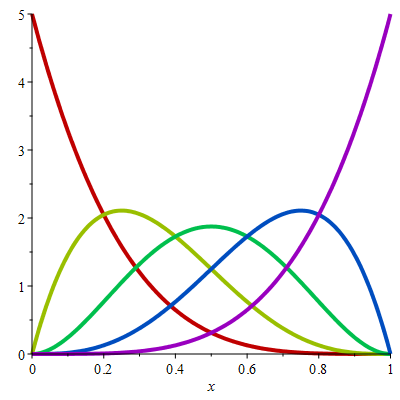
\includegraphics[width=0.45\textwidth]{images/beta5.png}\quad 
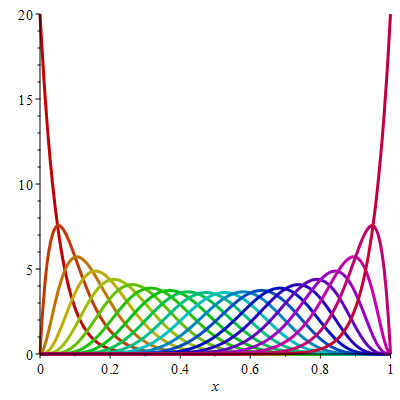
\includegraphics[width=0.45\textwidth]{images/beta20.png}
\caption{Pdf of position of $k$-th smallest of 5 (left) and 20 (right) independent, uniformly distributed numbers in $[0,1]$.  \label{kptpic}}
\end{figure}



\subsection{Exercises} 

\sse 
I toss a fair coin four times. Let $H$ be the number of heads I roll and let $C$ be the number of times (out of the three possible ones) that two consecutive coins tosses give the same result. 

Work out the $5 \times 3$ table of the joint probability mass function. From that compute the marginal distribution of $C$ and check that the marginal distribution of $H$ is binomial as you would expect.   Compute the expected value of $C$.  How could you compute the expected value of $C$ from the initial problem in your head? 
\end{e}

\sse
A unit length, thin rod breaks in two places, each break independently uniformly distributed on $[0,1]$. Let $a$ be a small number. Show that the probability that one of the three pieces into which the rod breaks has length less than $a$ is approximately $6a$ as $a \map 0$. 
\end{e}

\sss 
The relevant regions of the unit square are the four strips of width $a$ along each edge and a strip of width $\sqrt{a}$ around the $X_1 = X_2$ diagonal.  Ignoring overlaps (as $a \map 0$) they have a total area of $6 a$ 
\end{s}

\sse 
Compute the expected position of the $k$-th largest of $n$ independent, uniformly distributed numbers in $[0,1]$.  
\end{e}

\sss 
From the notes the pdf for the $k$th smallest of $n$ is 
\[
    f_{k,n}(x) = \frac{n!}{(k-1)! (n-k)!} x^{k-1} (1-x)^{n-k}. 
 \]
So its expected value is obtained by multiplying by $x$ and integrating: 
 \[
   \EE(X_{k,n}) = \int_0^1  \frac{n!}{(k-1)! (n-k)!} x^{k} (1-x)^{n-k}
   =  \frac{n!}{(k-1)! (n-k)!} \int_0^1   x^{k} (1-x)^{n-k}.
  \]
Using \S\ref{intfact} we evaluate the integral to be 
 \[
 \frac{n!}{(k-1)! (n-k)!} \, \frac{k! (n-k)!}{(n+1)!} = \frac{k}{n+1}.
 \]
\end{s}

\ssp 
Looking at the graphs in Figure~\ref{kptpic}, explain the following features, using mainly words rather than formulas. 
\begin{itemize}
\item Each picture is symmetric about the midpoint of the interval.
\item In the left-hand picture, the central blue-green graph is itself symmetric about the mid-point.
\item In both pictures, two of the graphs have non-zero values at one of the endpoints, but all the rest are zero at both end-points. 
\end{itemize}
\end{e}

\sss
\begin{itemize}
\item This is because the $k$-th smallest particle becomes the $k$-th largest particle if you reflect the interval in the mid-point. 
\item if there are an odd number $2k+1$ of particles, then the $k+1$-th particle reflects to itself under the symmetry just mentioned. 
\item The probability of having one particle in the interval $[0,\Delta t]$ is $n \Delta t$ as $\Delta t \map 0$.  So the corresponding distribution function approaches $n$ at the endpoints. But the probability of two points in such an interval is proportional to $(\Delta t)^2$ and so the distribution function must be zero at the end points. 
\end{itemize}
\end{s}




